\subsection{Implementations}

All powerflow solver code can be found in 
\texttt{lib/powerflow.py}, \texttt{lib/fastpf/powerflow.h}
\\ and
\texttt{lib/fastpf/powerflow.c}\\

The methods \texttt{solve\_powerflow\_gauss\_seidel()}
and \texttt{solve\_powerflow\_newton\_raphson()}
use python and numpy only and closely follow the mathematical formulations layed out above.\\

For the Gauss-Seidel method it is worth mentioning, that the Voltage result for each
node (\ref{eq:pf:gs_pf}) is immediately used to update the voltage vector. I.e. when $V_i^{(k+1)}$
is calculated the voltages $V_{j}^{(k+1)}$ where $j<i$ are already available and being used instead of
the old values $V_{j}^{(k)}$.\\

These methods where used as a baseline to access their performance. To identify where the biggest
speed-ups in performance could be gained timings where recorded for each of stages in the algorithm.
For a run of the python only Newton-Raphson timings to calculate the simbench grid shown in figure
\ref{fig:vep:simbench_node_types} are listed below:

\vspace{.5cm}

\begin{figure}[H]
    \begin{center}
        \begin{tabular}{ll}
            \textbf{Method section} & \textbf{Time (ms)}\\
            \hline
            Prepare matrices and vectors & 0.108\\
            Fill jacobian with zeros &  0.050\\
            Fill jacobian with values & 296.843\\
            Calculate Deltas &      0.067\\
            Invert Jacobian &      1.099\\
            Update voltage vector & 0.235\\
            \hline
            \textbf{Total} & \textbf{298.487}
        \end{tabular}
    \end{center}
\caption{Timings taken for different parts of the \texttt{solve\_powerflow\_newton\_raphson()} method}
\end{figure}
    
From this table it can immediately be seen, that the most important part
of the algorithm to optimize is filling the Jacobian with values. Thus, this
part was implemented in c using python c bindings to directly fill a numpy
matrix passed with values. This has the major advantage that only the most performance
critical code has to be implemented in c whilst everything else can be kept in python
for easy and quick development. Additionally, passing an existing matrix from python
means no additional memory allocations have to be done in c which is both good for performance 
and memory safety.\\
Taking the same timing for the c enhanced Newton-Raphson implementation yields the following:

\begin{figure}[H]
    \begin{center}
        \begin{tabular}{ll}
            \textbf{Method section} & \textbf{Time (ms)}\\
            \hline
            Prepare matrices and vectors & 0.232\\
            Fill jacobian with zeros &  0.051\\
            Fill jacobian with values & 0.436\\
            Calculate Deltas &      0.032\\
            Invert Jacobian &      1.493\\
            Update voltage vector & 0.016\\
            Finalize & 0.016\\
            \hline
            \textbf{Total} & \textbf{2.276}
        \end{tabular}
    \end{center}
\caption{Timings taken for different parts of the \texttt{fast\_newton\_raphson()} method}
\end{figure}

Using the new c method yields a considerable speed-up by more than ten times.\\

To unlock a further speed gain the matrices in use need to be examined closely. A normal admittance matrix has 
an entry for every possible combination of nodes $i$ and $j$, this means it has size $N^2$. However, if there is
no cable betewen $i$ and $j$ this entry is zero. As a lot of these cables do not exist a lot of the entries are zero
and the admittance matrix is sparse.
As can be seen from equation \ref{eq:pf:nr_pf_jacobi} as well as \ref{eq:pf:nr_pf_p} and \ref{eq:pf:nr_pf_q} the entries
in the Jacobian are also zero if a given entry $y_{ij}$ is zero in the admittance matrix.\\
Just iterating over these zero entries or doing multiplications of zero values wastes considerable processor time. On top
the large matrices take up a lot of memory. This problem can be solved by specifically using
a sparse matrix library like \textit{scipy.sparse}\autocite{2020SciPy-NMeth}. The library offers
data types that only store non-zero elements within the matrix as well as solvers that can operate
efficiently on these types.\\
Using the sparse library as well as implementing c code that operates on this matrix type a
further performance gain is possible:

\begin{figure}[H]
    \begin{center}
        \begin{tabular}{ll}
            \textbf{Method section} & \textbf{Time (ms)}\\
            \hline
            Prepare matrices and vectors & 0.075\\
            Fill power vec. with zeros &  0.007\\
            Fill jacobian with values & 0.179\\
            Calculate Deltas &      0.024\\
            Invert Jacobian &      0.452\\
            Update voltage vector & 0.015\\
            Finalize & 0.013\\
            \hline
            \textbf{Total} & \textbf{0.765}
        \end{tabular}
    \end{center}
\caption{Timings taken for different parts of the \texttt{fast\_newton\_raphson\_sparse()} method}
\end{figure}

\subsection{Validation}

\subsubsection{Simple 3 node grid}

\begin{figure}[H]
    \centering
    \begin{tikzpicture}[scale=1]


    % Slack
    \draw[line width=.8mm] (-4, -1) coordinate(s1) -- ++(0, 2.5) coordinate(e1) node(slack)[above]{1: Slack Node};
    \node (voltage_label) at ($(s1) - (.2, 0)$)[left] {$V_1 = 1.05 pu$};

    % Load 1
    \draw[line width=.8mm] (4, -1) coordinate(s2) -- ++(0, 2.5) coordinate(e2) node(slack)[above]{2: Prosumer};
    \node (q_label1) at ($(s2) + (.2, 0)$)[left][right] {$Q = 110.2Mvar$};
    \node (p_label1) at ([yshift=2mm]q_label1)[above] {$P = 256.6MW$};

    % Load 2
    \draw[line width=.8mm, name path=l2] (-1.5, -2) coordinate(s3) -- ++(3, 0) coordinate(e3);
    \node(slack) at ($(s3) - (0, .3)$)[left]{3: Prosmuer};
    \node(p_label2) at ($(e3) - (0, .3)$)[right]{$P = 138.6MW$};
    \node(q_label2) at ([yshift=-2mm]p_label2)[below]{$Q = 45.2 Mvar$};

    % Lines
    \draw[line width=.5mm] ($(e1) - (0, .7)$) -- ($(e2) - (0, .7)$) node[pos=.5](l1_midpoint){};
    \node(line_lbl_1) at (l1_midpoint)[above]{$y_{12} = 10-j20$};

    \draw[line width=.5mm] ($(s1) + (0, .7)$) -- ++(3, 0) coordinate(l2_end) node[pos=.5](l2_midpoint){};
    \node(line_lbl_2) at (l2_midpoint)[above]{$y_{13} = 10-j30$};

    \path[name path=intercept] (l2_end) -- ++(0, -4);
    \draw[
        line width=.5mm,
        name intersections={of=intercept and l2}
    ] (l2_end) to (intersection-1);

    \draw[line width=.5mm] ($(s2) + (0, .7)$) -- ++(-3, 0) coordinate(l3_end) node[pos=.5](l3_midpoint){};
    \node(line_lbl_3) at (l3_midpoint)[above]{$y_{23} = 16-j32$};

    \path[name path=intercept2] (l3_end) -- ++(0, -4);
    \draw[
        line width=.5mm,
        name intersections={of=intercept2 and l2}
    ] (l3_end) to (intersection-1);

  \end{tikzpicture}
    \caption{
        A simple 3 node system taken from \textit{Power System Analysis}\autocite{power_system_analysis}.
        Admittances $y_{ij}$ are in $pu$ (power unit) on a 100-MVA base.
        $P$ and $Q$ of prosumers are positive for consumption and negative for production.
    }
    \label{fig:pf:3_node_system}
\end{figure}


Fast powerflow is good, but no use if it is not correct. For validation
the solvers are compared against the system shown in figure \ref{fig:pf:3_node_system} and results
provided in \textit{Power System Analysis}\autocite{power_system_analysis}.

\begin{figure}[H]
    \begin{center}
        \begin{tabular}{m{3cm} | m{2.5cm} m{2.5cm} m{2.5cm} m{2.5cm}}
            Method & Slack real Power $P_1$ (MW) & Slack reactive Power $Q_1$ (Mvar) & Node 2 Voltage $V_2$ ($pu$) & Node 3 Voltage $V_2$ ($pu$)\\
            \hline
            Gauss-Seidel in \textit{Power System Analysis}\autocite{power_system_analysis} & $409.5$ & $189$ & $0.9800 - j0.0600$ & $1.0000 - j0.0500$\\
            \hline
            Own Gauss-Seidel implementation & 409.4 & 188.9 & $0.9800-j0.0600$ & $1.0000 - j0.0500$ \\
            \hline
            Own Newton-Raphson implementation (basic) & 409.5 & 189 & $0.9800-j0.0600$ & $1.0000 - j0.0500$ \\
        \end{tabular}
    \end{center}
    \caption{Results obtained through different methods for the grid shown in figure \ref{fig:pf:3_node_system}}
\end{figure}

The table above shows that the results obtained with our own Gauss-Seidel and Newton-Raphson
implementations agree with each other and with the values calculated in \textit{Power System Analysis}\autocite{power_system_analysis}. The accelerated
Newton-Raphson methods have also been compared with the values shown above, they are exactly equal to the values 
for the basic Newton-Raphson implementation

\subsubsection{Pandapower}

A second validation was carried out against the widely used open source package
\textit{panadapower}\autocite{pandapower2018}. The \textit{Simbench} grid
introduced in \autoref{fig:vep:simbench_node_types} was used here. Values
produced by \textit{panadapower} and our implementation agree exactly.

\subsection{Performance}


\begin{figure}[H]
    \centering
    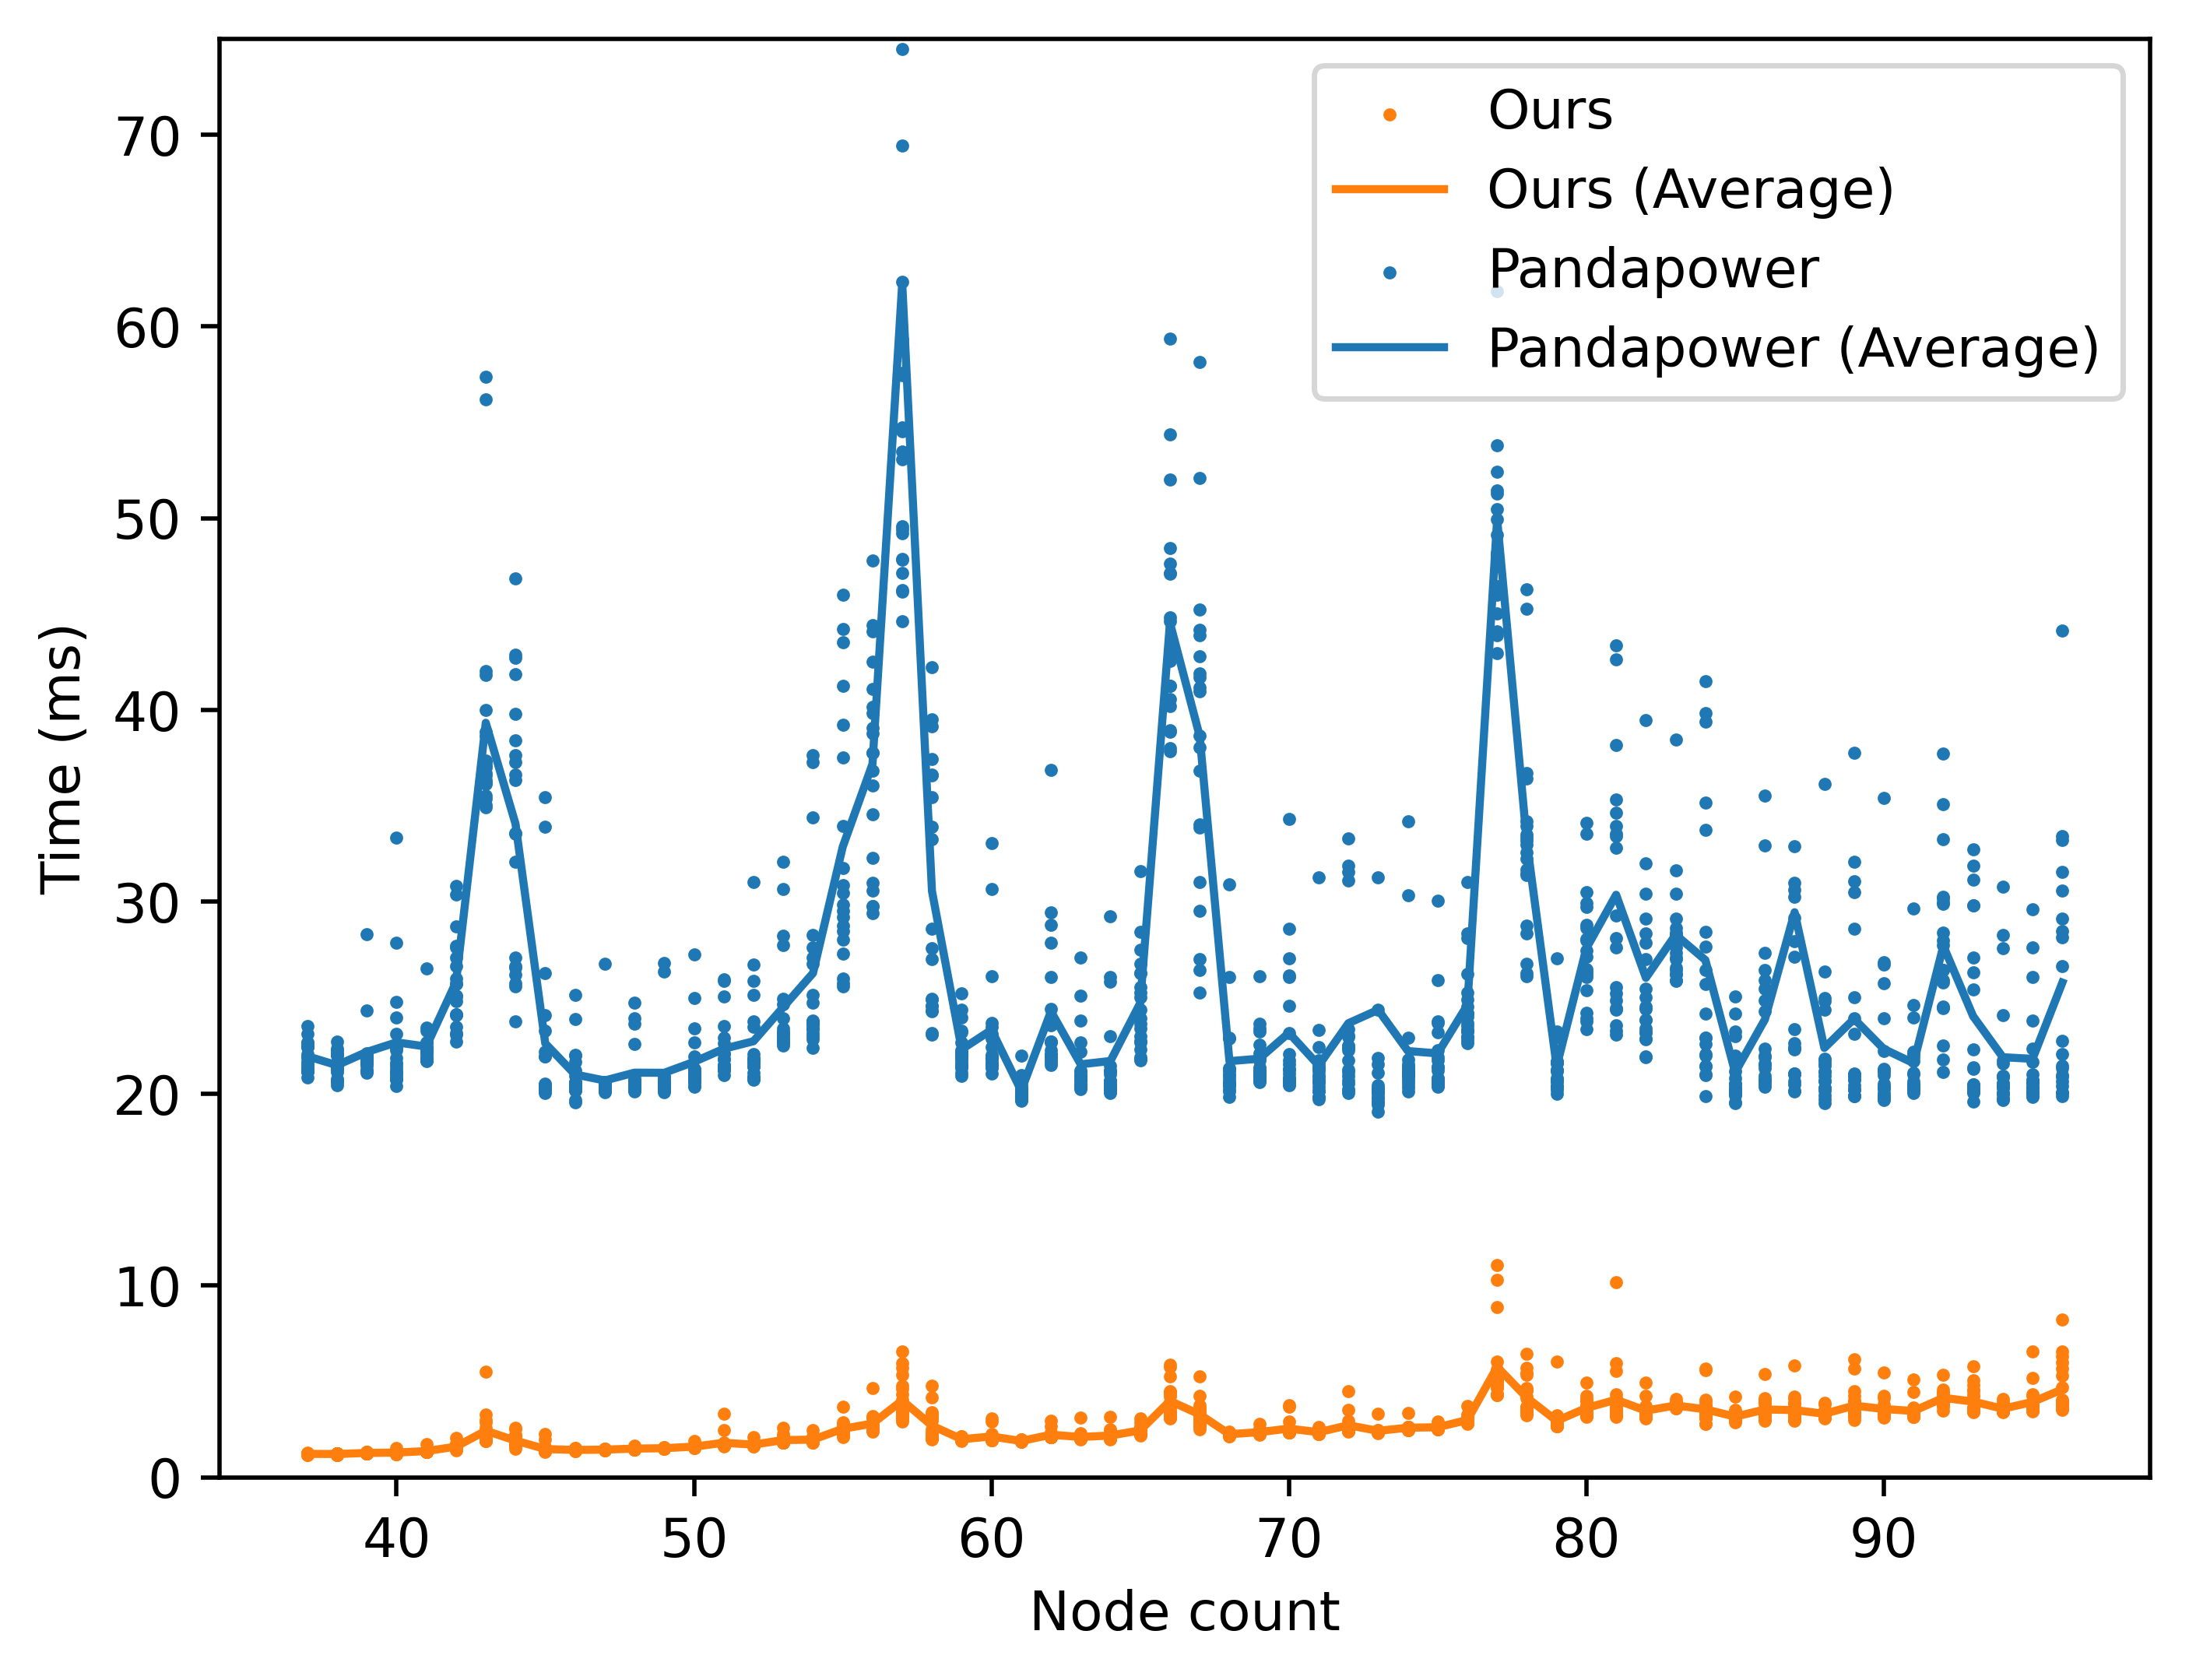
\includegraphics[width=.65\linewidth]{img/benchmark/pandapower_avg.png}
    \caption{
        Iteration time of \textit{pandapower}\autocite{pandapower2018} Newton-Raphson and our implementation of
        Newton-Raphson vs. grid size. 20 samples taken for every grid size. Simbench
        grid (\autoref{fig:vep:simbench_node_types}) used and shrunk by cutting
        away outer nodes. Admittance matrix creation and result power vector creation 
        is included in the timings for our method as \textit{pandapower} is also calculating
        these values
    }
    \label{fig:pf:benchmark}
\end{figure}

\autoref{fig:pf:benchmark} shows the performance difference between our method and \textit{pandapower}.
Our method is up to an order of magnitude faster than \textit{pandapower} and has better timing
consistency. Egor Grishin et. al. show that \textit{pandapower} is among the faster power flow
implementations available in python\autocite{newton_raphson_python}. Our method should therefore
be as fast or faster than the fastest available python Newton-Raphson implementations.\\
\\
That this is the case will partially be due to the vastly reduced feature set of our method
(it just calculates the voltage vector based on the admittance matrix). However, to write
something like a switch state optimizer, this is all that is needed, and the additional
performance makes a big difference in how many switch states can be assessed in a given time.
